\section{Search Algorithms} % (fold)
\label{sec:search_algorithms}
Six search methods were implemented to provide solutions to the \gls{rnp}, three of which are \gls{informed} methods and three \gls{uninformed} methods. Each was tested using a combination of unit testing and statistical experiments outlined in subsection~\ref{sub:methodology}. Furthermore, while this section contains a high-level discussion of the qualities and draw-backs of each search method used, an analysis of their optimality, completeness, time, and space complexity is described in-depth in section~\ref{sec:research} as a component of this reports research initiative.

\subsection{\texorpdfstring{\acrfull{as}}{A*}} % (fold)
\label{sub:as}
A* is an \gls{informed} search method that stores its frontier in a priority queue structure sorted by best node first, as determined by the nodes \textit{evaluation function} $f(n)$ which evaluates the cost of reaching a given node $n$. For A*, $f$ is defined as the cost to reach $n$ from the starting node along the current path - $g(n)$ and its heuristic function $h(n)$ which provides an estimation of the cost of reaching the goal. A requirement for A* to be correctly implemented is that $h$ be \gls{admissible}, that is it never overestimates the quality of a path or node. In the context of the RNP, as the environment is a 2D grid, an admissible heuristic can be achieved by simply measuring the distance from the current node using either euclidean distance, calculated by $\sqrt{(x_1 - x_2)^2 + (y_1 - y_2)^2}$, or using a 'city-block' distance (the amount of nodes traversed without diagonal movements) referred to as \textit{manhattan} distance, calculated by $\left|x_1 - x_2\right| + \left|y_1 - y_2\right|$. A* is both complete and optimal \parencite[104]{astar}, as well as efficient in terms of both time and space complexity. For this reason it's used as a comparison for all subsequent search methods described here.
% subsection as (end)

\subsection{\texorpdfstring{\acrfull{bfs}}{BFS}} % (fold)
\label{sub:bfs}
Breadth-First search is an uninformed search method that uses a \acrfull{fifo} as its frontier, resulting in the shallowest node encountered expanded first. As a consequence of this expansion method, BFS is \gls{complete} in all spaces as eventually every node in the search space will be expanded. Furthermore, BFS is technically \gls{optimal} when the step cost of a node is non-decreasing and equivalent to it's depth \parencite[82]{aiama}. However, while BFS is both complete and optimal it can be inefficient in terms of both memory and time. As BFS eventually analyses every node in the search space, larger grids can increase its memory consumption much more than other algorithms, as demonstrated in figure ~\ref{fig:expanded_relationship}. Furthermore, it's runtime increases proportional the time it takes to scan it's list of neighbors \parencite[597]{introalgos}, which will always be the amount of nodes that exist at depth $d$ extending from the start, minus the ones explored.
% subsection bfs (end)

\begin{figure}[H]
	\label{fig:expanded_relationship}
	\centerline{
		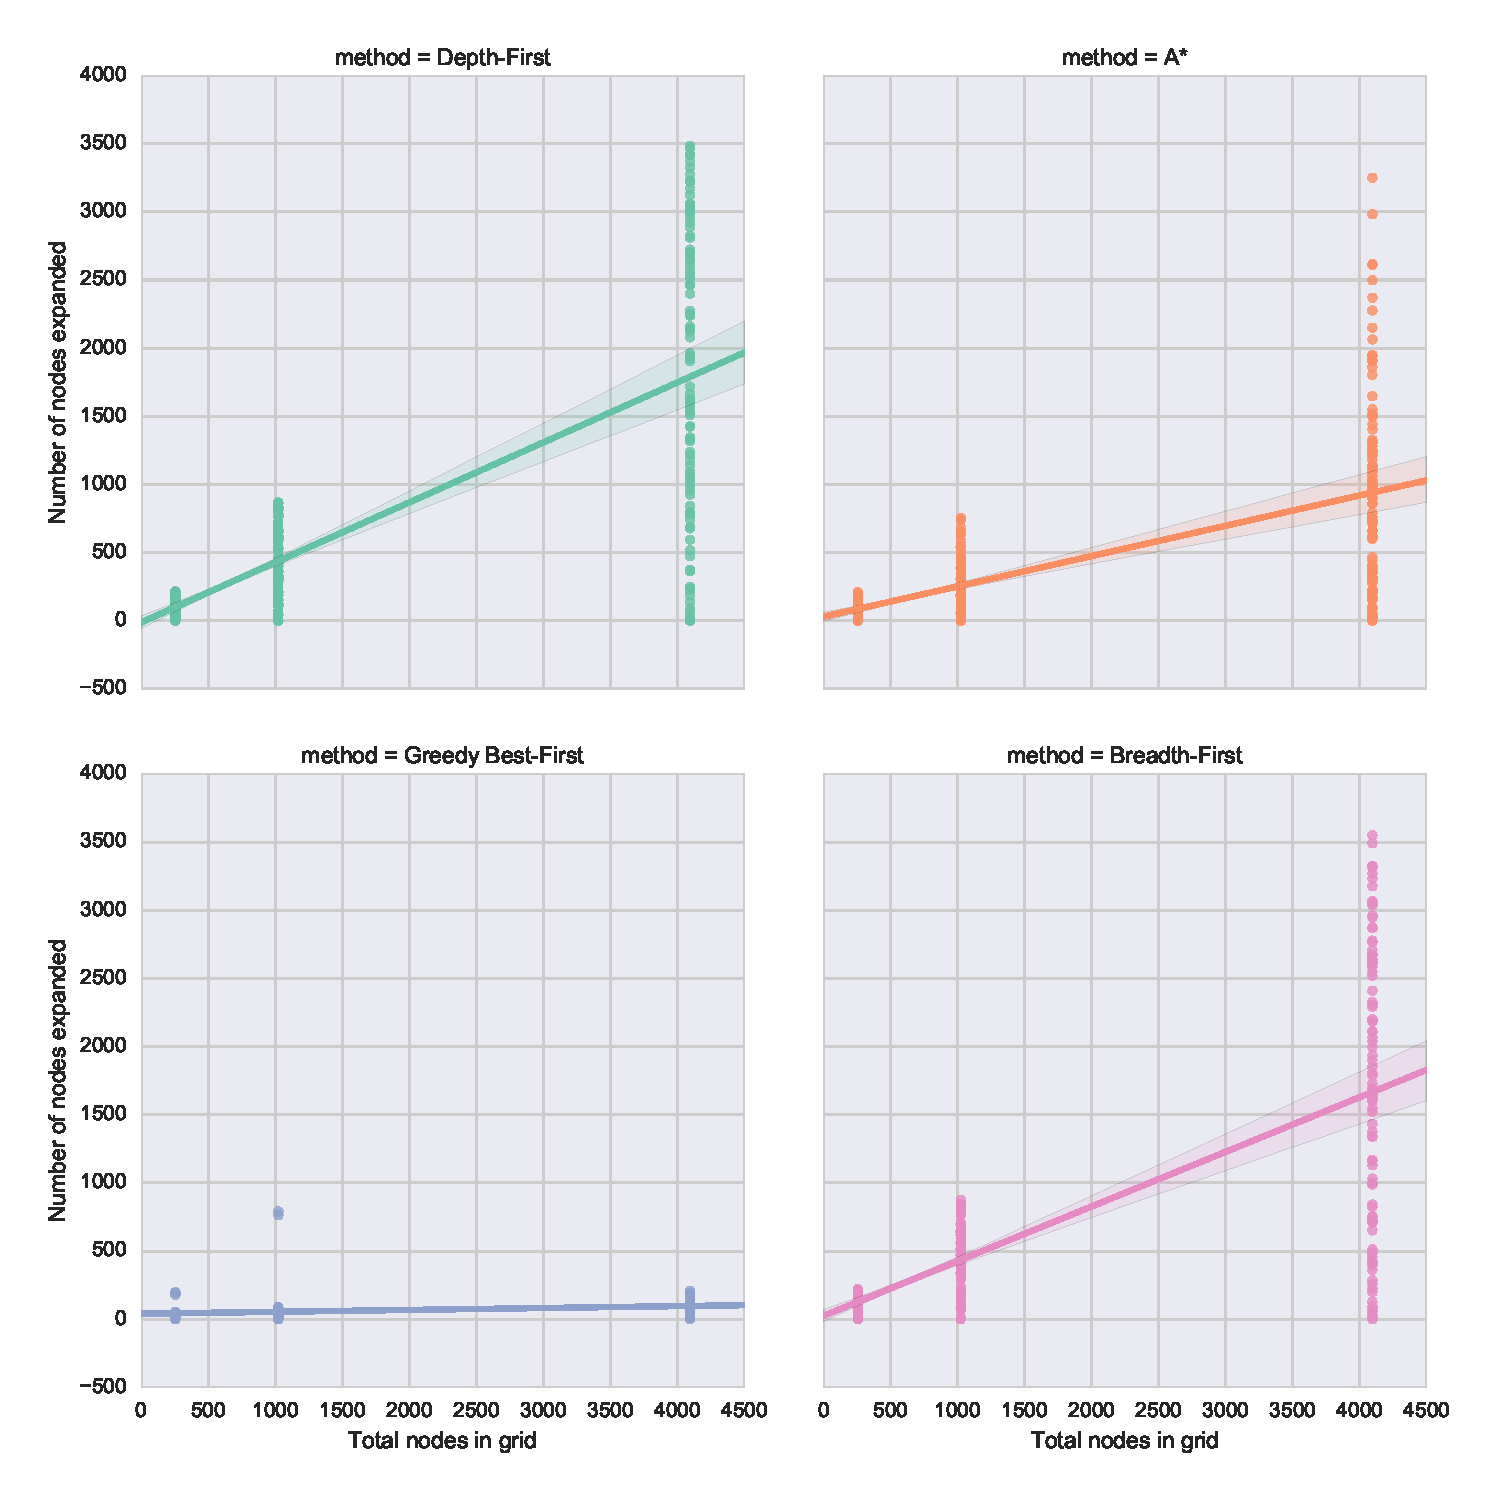
\includegraphics[width=0.75\textwidth]{Resources/Stats/expanded_relationship.pdf}
	}
	\caption{Linear relationship between size of RNP grid and the number of nodes expanded for each search algorithm}
\end{figure}

\subsection{\texorpdfstring{\acrfull{dfs}}{DFS}} % (fold)
\label{sub:dfs}
Depth-First search is an uninformed search method that uses a \acrfull{lifo} as its frontier. It will always follow the last-encountered node until it hits either a \gls{leaf} or the goal. In theory this poses obvious advantages over BFS, namely in terms of its memory usage - as it only ever contains the current path and each of the path nodes immediate neighbors - however, DFS has many disadvantages. Firstly, it's non-optimal - for example, if DFS chooses to expand a node to its left (based a pre-defined order of expansion), it will follow that path even if the goal was located one node to the right. In the worst case, this could result in DFS following the longest possible path possible rather than a shorter alternative. Figure~\ref{fig:dfs_bfs_length} highlights this problem, showing the difference in distribution of path lengths between BFS and DFS across 300 randomly generated grids.
% subsection dfs (end)

\begin{figure}[H]
	\hfill
	\subfigure[BFS]{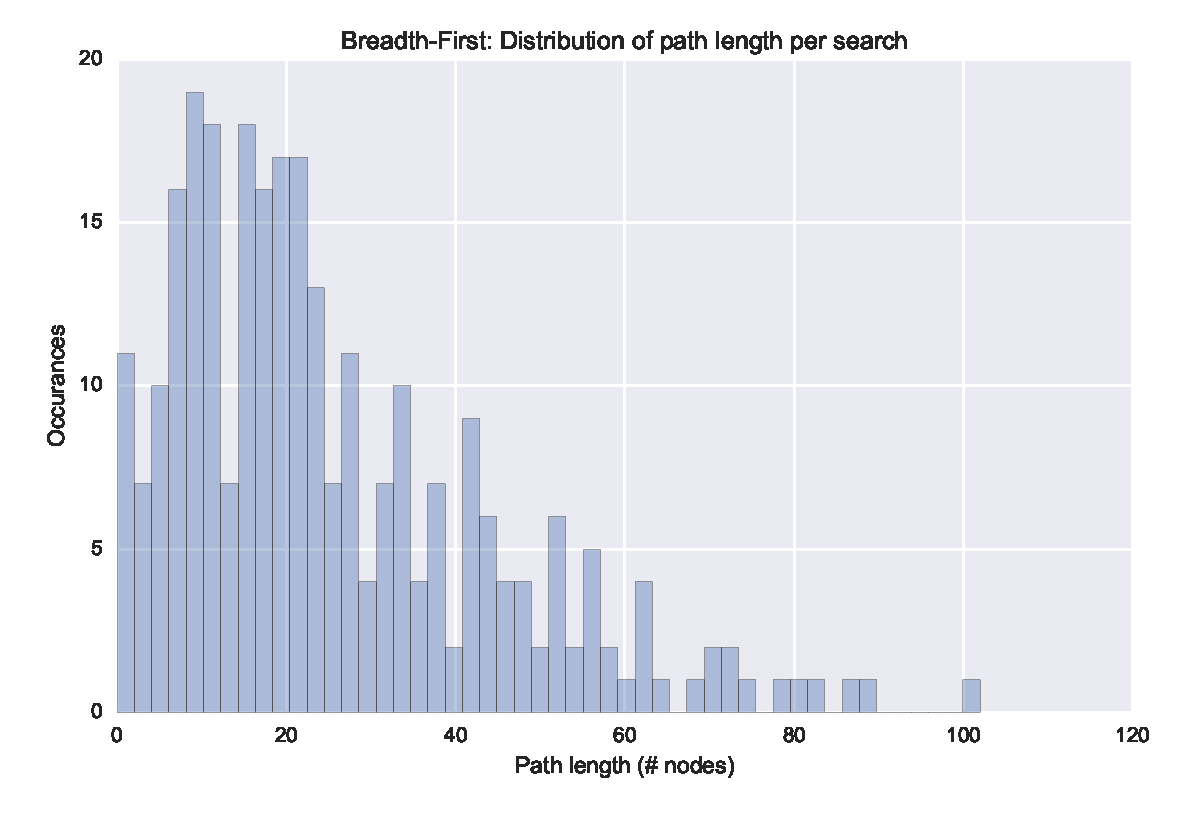
\includegraphics[width=0.45\textwidth]{Resources/Stats/Breadth-First-hist-path_length.pdf}}
	\hfill
	\subfigure[DFS]{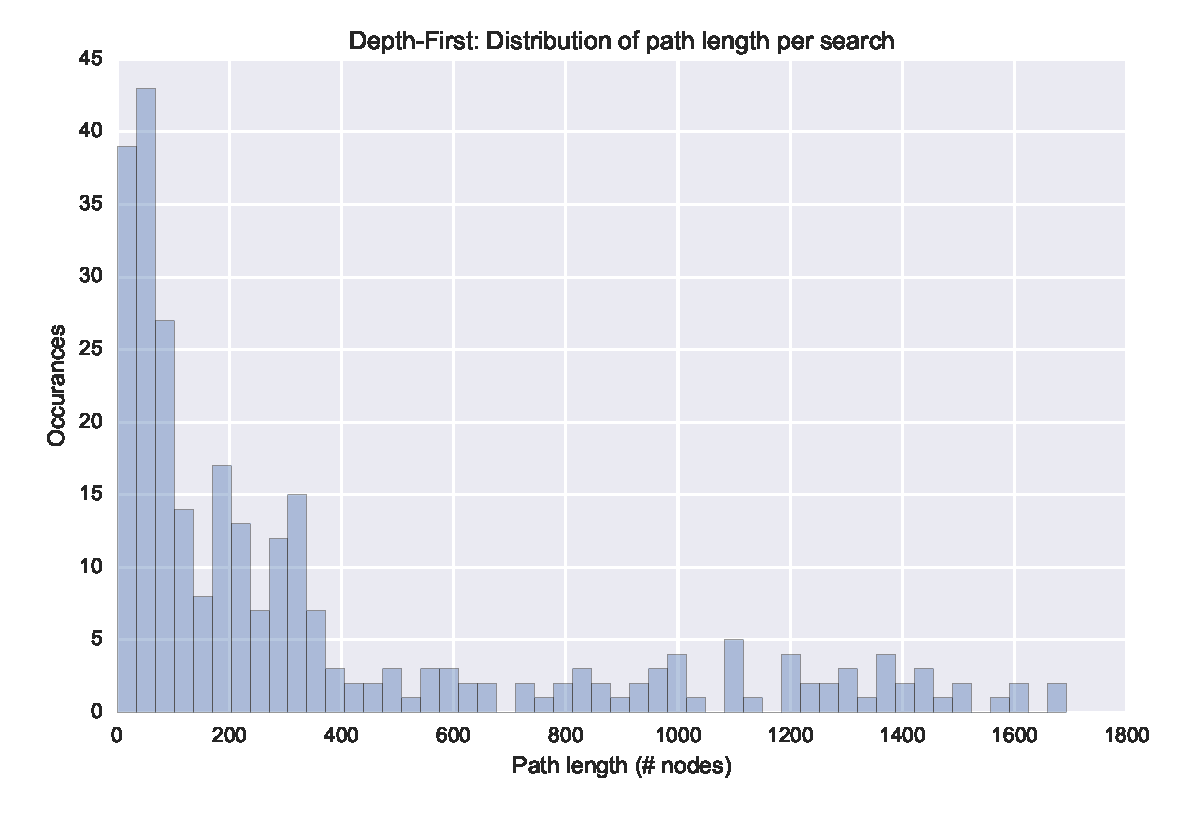
\includegraphics[width=0.45\textwidth]{Resources/Stats/Depth-First-hist-path_length.pdf}}
	\caption{Comparison between the distributions of total path length for Breadth-First Search and Depth-First Search}
	\label{fig:dfs_bfs_length}
\end{figure}

Furthermore, DFS is only complete in graph-based searches whereas the tree-based version is \textit{incomplete} \parencite[86]{aiama}. Both of these factors result in large runtime consequences, especially as the search space increases in size as demonstrated in figure %TODO: put figure ref here

\subsection{\texorpdfstring{\acrfull{gbfs}}{GBFS}} % (fold)
\label{sub:gbfs}
Greedy Best-First is an \textit{informed} search method which, like all informed methods outlined in this report, uses a priority queue frontier ordered by lowest $f$ value. In contrast to A*, GBFS expands the node that is closest to the goal first, therefore it's evaluation is $f(n)=h(n)$. GBFS, in contrast to A*, is not optimal nor is it complete \parencite{aiasa}, this is because its heuristic is not \textit{admissible} due to often overestimating the quality of a node, for example in scenarios when the goal is behind a wall but unreachable, the node closest will be evaluated as the best neighbor when it isn't. However, often GBFS can return a \textit{close to optimal path} while expanding less nodes in a faster time than other search methods, demonstrated in figure~\ref{fig:mean_runtime_expanded}.

\begin{figure}[H]
	\hfill
	\subfigure[Mean run-times]{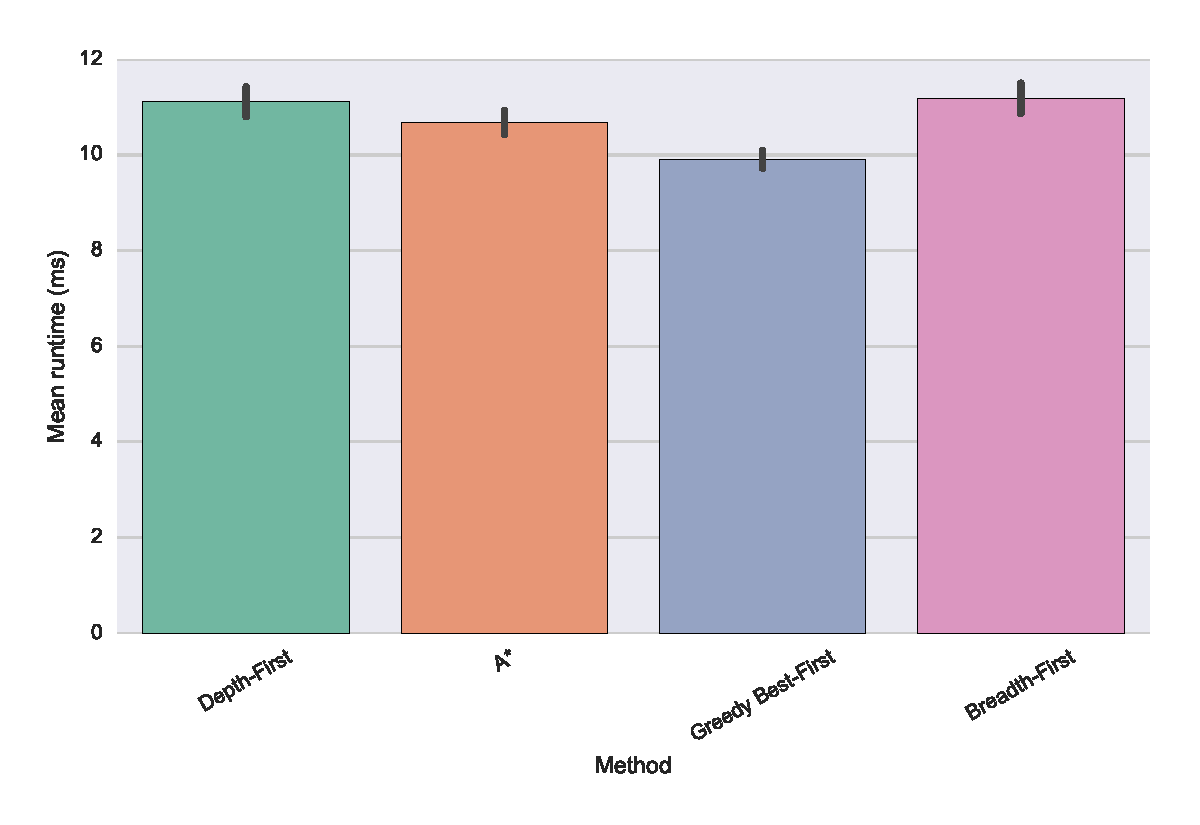
\includegraphics[width=0.45\textwidth]{Resources/Stats/runtime_bars.pdf}}
	\hfill
	\subfigure[Mean nodes expanded]{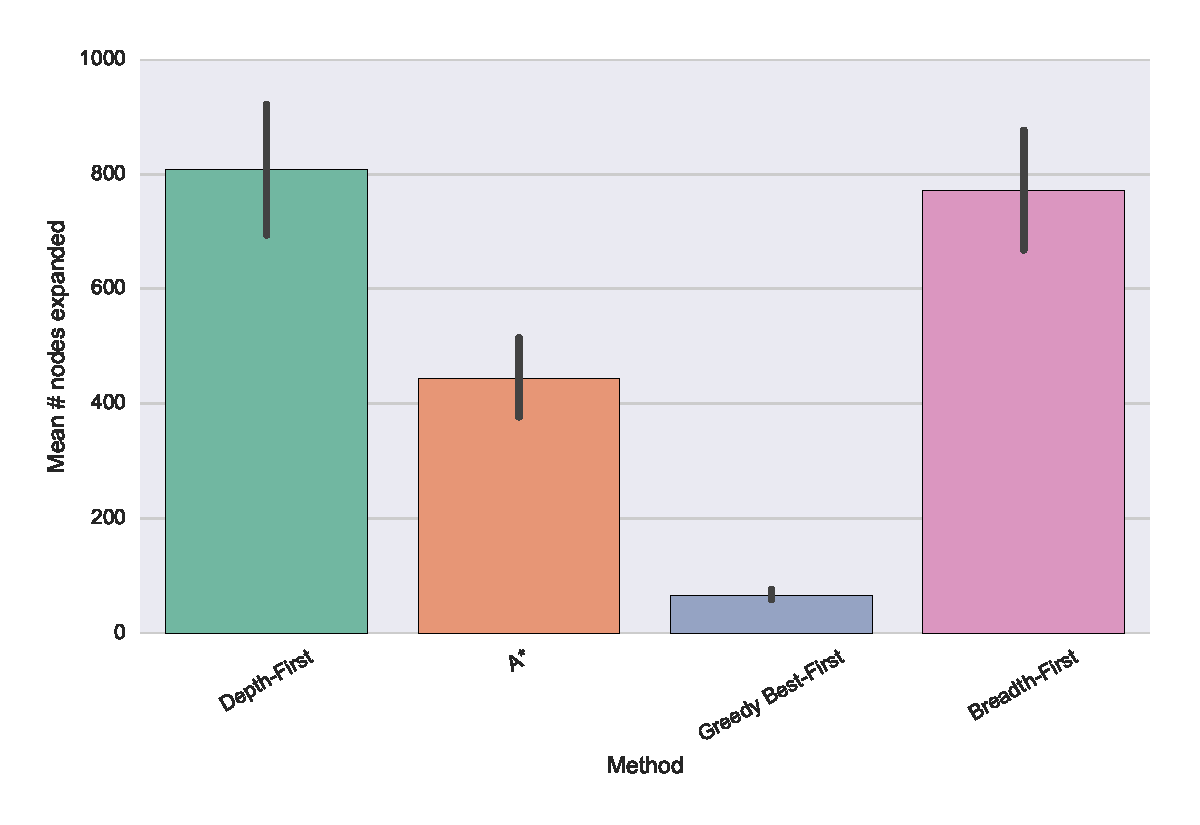
\includegraphics[width=0.45\textwidth]{Resources/Stats/expanded_bars.pdf}}
	\caption{The mean number of nodes expanded and mean run-time for the non-custom search methods}
	\label{fig:mean_runtime_expanded}
\end{figure}

% subsection gbfs (end)

\subsection{\texorpdfstring{\acrfull{iddfs}(\texttt{CUS1})}{IDDFS}} % (fold)
\label{sub:iddfs}
Iterative Deepening Depth-First search is an improved version of regular depth-first search uninformed search which executes DFS until either the goal is encountered or some depth-limit $\ell$ is reached, signaling a cutoff upon which the search tree is cleared, increasing $\ell$ by 1 and running the algorithm again, running iterations of DFS until the goal is found. This method aims to combine the best qualities of DFS and BFS, taking the limited space requirements of DFS and combining it with the completeness and optimality of BFS.
% subsection iddfs (end)

\subsection{\texorpdfstring{\acrfull{ida}(\texttt{CUS2})}{IDA}} % (fold)
\label{sub:texorpdfstring}
Iterative Deepening A* is a search method that attempt to improve the memory requirements of A*. It is similar to IDDFS in its methodology, except for what is used as $\ell$ for the current iteration. A cutoff is reached when the current nodes $f$ cost exceeds the current $\ell$ value, upon which $\ell$ is increased to be equal to that nodes $f$, the search tree cleared and another iteration begun. In a sample of 300 randomly generated grids of differing sizes, IDA* cut down the mean amount of nodes expanded by approximately 50 nodes as demonstrated in figure~\ref{fig:idas_as_expanded}.

\begin{figure}[H]
	\label{fig:idas_as_expanded}
	\centerline{
		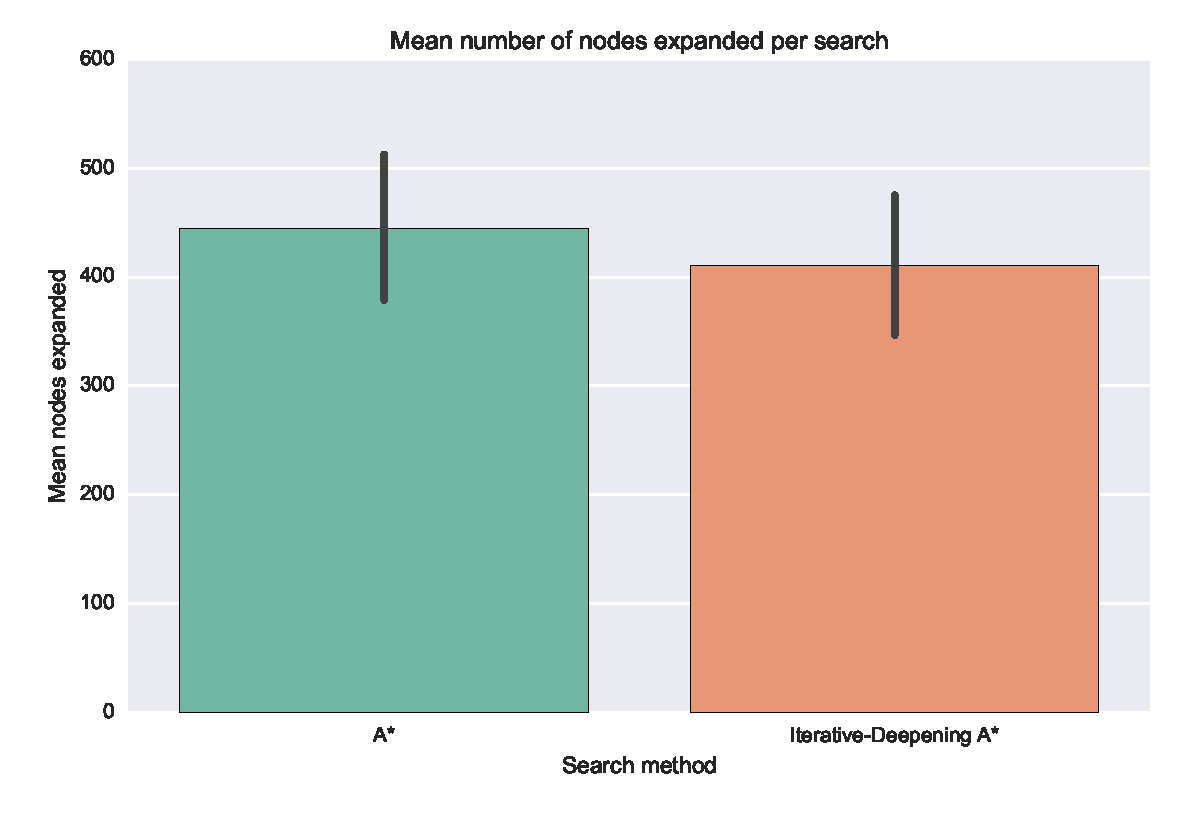
\includegraphics[width=0.7\textwidth]{Resources/Stats/Iterative-Deepening A*-bar-nodes_expanded.pdf}
	}
	\caption{Comparison of mean number of nodes expanded per search between A* and IDA*}
\end{figure}

However, while memory requirements are improved, on graph-based searches such as the RNP IDA*'s tendency to analyze the same state for different depths in a standard implementation showed an increase of approximately 800\textit{ms} per search as shown in figure~\ref{fig:idas_as_runtime}.

\begin{figure}[H]
	\label{fig:idas_as_runtime}
	\centerline{
		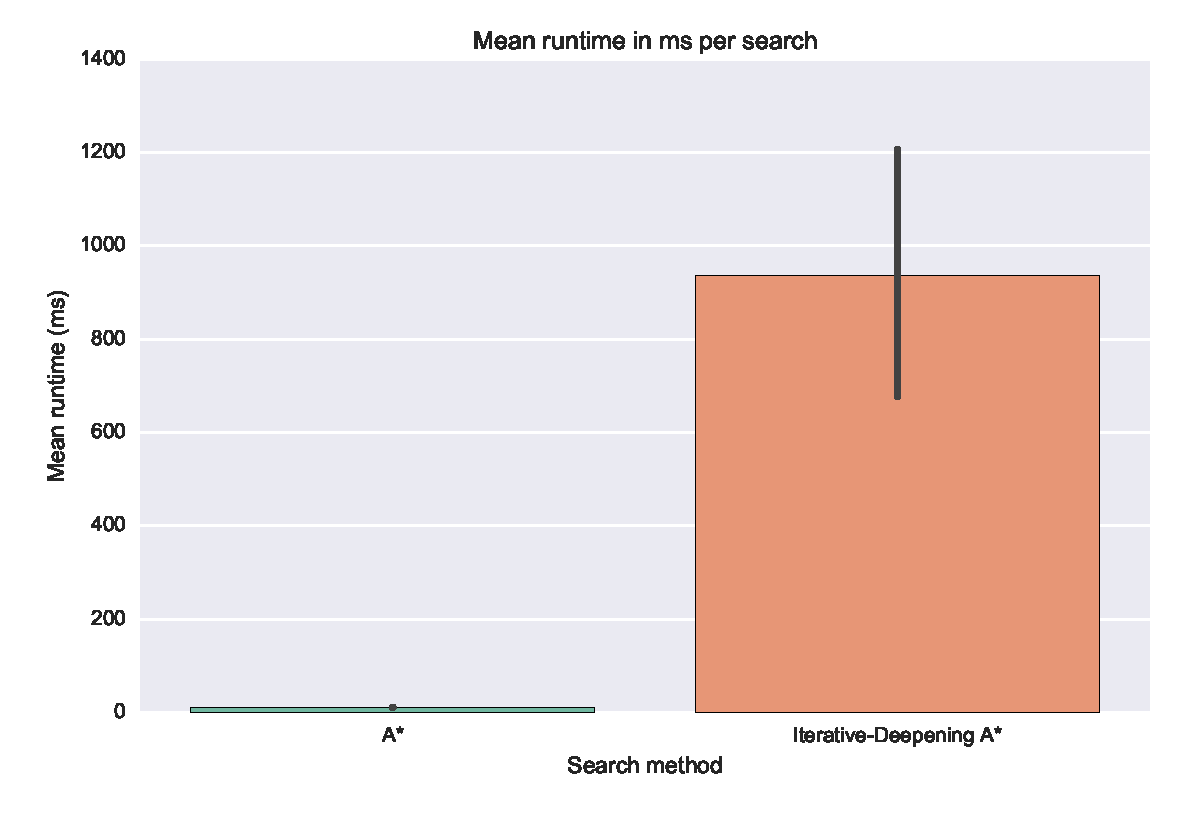
\includegraphics[width=0.7\textwidth]{Resources/Stats/Iterative-Deepening A*-bar-execution_time.pdf}
	}
	\caption{Comparison of mean run-time per search between A* and IDA*}
\end{figure}

However, it's important to note that the implementation described in section~\ref{sec:implementation} does not make much effort to track repeated states in graph-based problems and IDA* is technically as efficient as A* given the right implementation \parencite{idas}.

% subsection texorpdfstring (end)

% section search_algorithms (end)
